\documentclass[12pt,a4paper]{article}

% Encoding and fonts
\usepackage[utf8]{inputenc}
\usepackage[T1]{fontenc}
\usepackage{lmodern}

% Page layout
\usepackage{geometry}
\geometry{
    a4paper,
    top=25mm,
    bottom=25mm,
    left=25mm,
    right=25mm
}

% Line spacing
\usepackage{setspace}
\setstretch{1.15}

% Figures and tables
\usepackage{graphicx}
\usepackage{float}

% Mathematics
\usepackage{amsmath}
\usepackage{amssymb}
\usepackage{amsthm}

% Theorem formatting
\newtheoremstyle{style}
    {0.5cm}
    {-0.8cm}
    {}
    {}
    {\normalfont\bfseries}
    {}
    { }
    {\thmname{#1}\thmnumber{ #2}}

\theoremstyle{style}
\newtheorem{example}{Example}[section]
\newtheorem{formula}{Formula}[section]

% References
\usepackage{natbib}

% Captions
\usepackage{caption}
\captionsetup{
    font=small,
    labelfont=bf,
    labelsep=period,
    justification=centering
}

% Table of contents depth
\setcounter{tocdepth}{3}

% Horizontal rule command
\newcommand{\HRule}{\rule{\linewidth}{0.5mm}}

% Paragraph formatting
\setlength{\parindent}{0pt}
\setlength{\parskip}{0.8em}

% Hyperlinks
\usepackage[hidelinks]{hyperref}


\begin{document}


% Title page
\begin{titlepage}
\centering


\includegraphics[width=0.15\textwidth]{eule}

\vspace{0.8cm}

{\LARGE\scshape Saarland University\par}
\vspace{0.2cm}
{\large Faculty of Mathematics and Computer Science\par}

\vfill

{\Large Project Seminar Report\par}

\vspace{0.7cm}

{\Huge\bfseries
Auditing Platform Algorithms Using the Pro-Choice / Pro-Life Posts on Instagram\\[0.2em]
in Social Media
\par}

\vspace{0.8cm}

{\Large
Project Seminar Data Science and Artificial Intelligence
\par}

\vfill

\begin{tabular}{c}
Dr. Till Koebe\\[0.2cm]
Prof. Dr. Ingmar Weber\\[0.2cm]
Brahmani Nutakki
\end{tabular}

\vspace{1.5cm}

\begin{tabular}{cc}
\textbf{Shergo Shami} &
\textbf{Karl Kevin Ondobo Enama} \\[0.3em]
Matriculation No. 7023158 &
Matriculation No. 7032903
\end{tabular}

\vfill

{\large July 31, 2026}

\end{titlepage}

\thispagestyle{empty}


% Abstract
\clearpage

\begin{center}
    {\Large\bfseries Abstract}
\end{center}

\vspace{1cm}

\begin{singlespace}

Social media platforms increasingly use algorithmic ranking and recommendation systems to determine which content users encounter and how they interact with it. While these systems are designed to personalize experiences, they may also contribute to differences in the information environments and discussion spaces experienced by different users. Understanding the mechanisms behind these differences is essential for assessing the effects of personalization on online discourse.

This research investigates the factors that contribute to divergence in social media interactions, focusing on discussions around polarized topics. The study uses data collected from controlled user profiles with different demographic and ideological characteristics to examine how variations between users are reflected in their exposure patterns, engagement behaviours, and interactions with opposing viewpoints.

A combination of exploratory analysis, feature engineering, and statistical modelling is employed to identify the characteristics associated with divergent user experiences. The analysis evaluates the influence of content properties, temporal dynamics, engagement signals, and user-level attributes on measures of interaction divergence. Regression models are used to quantify the relationship between these factors and differences observed across user profiles.

The results provide a data-driven examination of how personalization mechanisms and user characteristics shape online interaction environments. By identifying the factors associated with divergent experiences, this study contributes to the understanding of algorithmic influence, information exposure, and polarization dynamics in social media platforms.

\end{singlespace}


% Table of contents
\clearpage

\thispagestyle{empty}

\tableofcontents


% Main document
\clearpage

\pagenumbering{arabic}
\setcounter{page}{1}


\section{Introduction}

\subsection{Background and Motivation}

Social media platforms have emerged as central spaces for public discourse, providing individuals with unprecedented opportunities to express opinions, exchange perspectives, and participate in debates surrounding contentious social and political issues. Among these platforms, Instagram (one of the world’s largest social networks, with over one billion monthly active users ) serves as a dynamic environment where diverse communities engage with and respond to shared content. Examining how users with different ideological orientations and gender identities interact within these digital spaces is essential for understanding the mechanisms underlying online polarization, opinion formation, and the diffusion of information in contemporary society.

\subsection{Dataset Overview}

The dataset captures the dynamics of one of the most polarizing contemporary debates: The Abortion Debate, A Clash of Rights: Whose Body? Whose Choice? Whose Life? \\
The posts were systematically sampled across six user categories defined by the intersection of gender and ideological stance: Female/Male × Neutral/Pro-Choice/Pro-Life, with 612 posts collected from each category. This balanced sampling design enables a systematic comparison of divergence patterns across identity-based and ideological dimensions.


The dataset is organized into six equally represented user groups:
\begin{itemize}
    \item female\_neutral
    \item female\_prochoice
    \item female\_prolife
    \item male\_neutral
    \item male\_prochoice
    \item male\_prolife
\end{itemize}

Each category contains exactly 612 posts, ensuring a balanced representation across both gender and ideological dimensions.

\begin{figure}[!htbp]
\centering
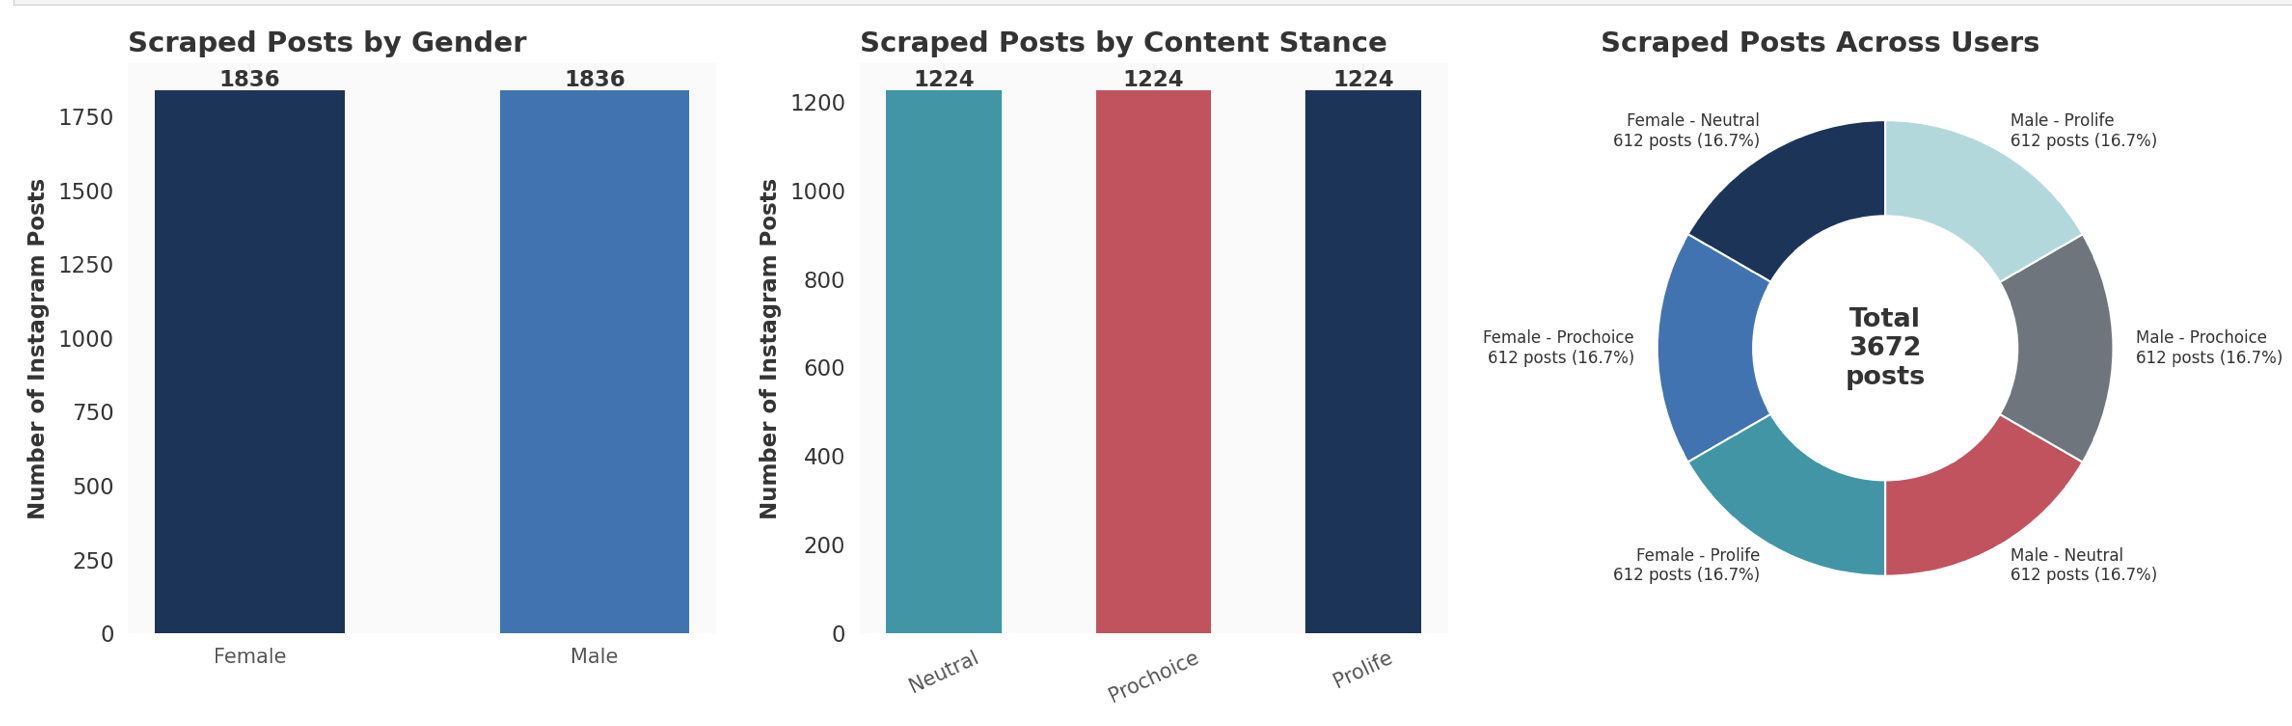
\includegraphics[width=0.9\textwidth]{plots/posts_distribution.png}
\caption{Distribution of posts across gender and stance categories.}
\label{fig:posts_distribution}
\end{figure}


Across all posts, the dataset records 5,721,684 likes and 218,619 comments. Engagement is highly skewed, with posts receiving an average of 9,349 likes and 357 comments, compared to medians of 866 likes and 53 comments, respectively. This difference highlights substantial variation in engagement levels across posts.

\begin{figure}[!htbp]
\centering
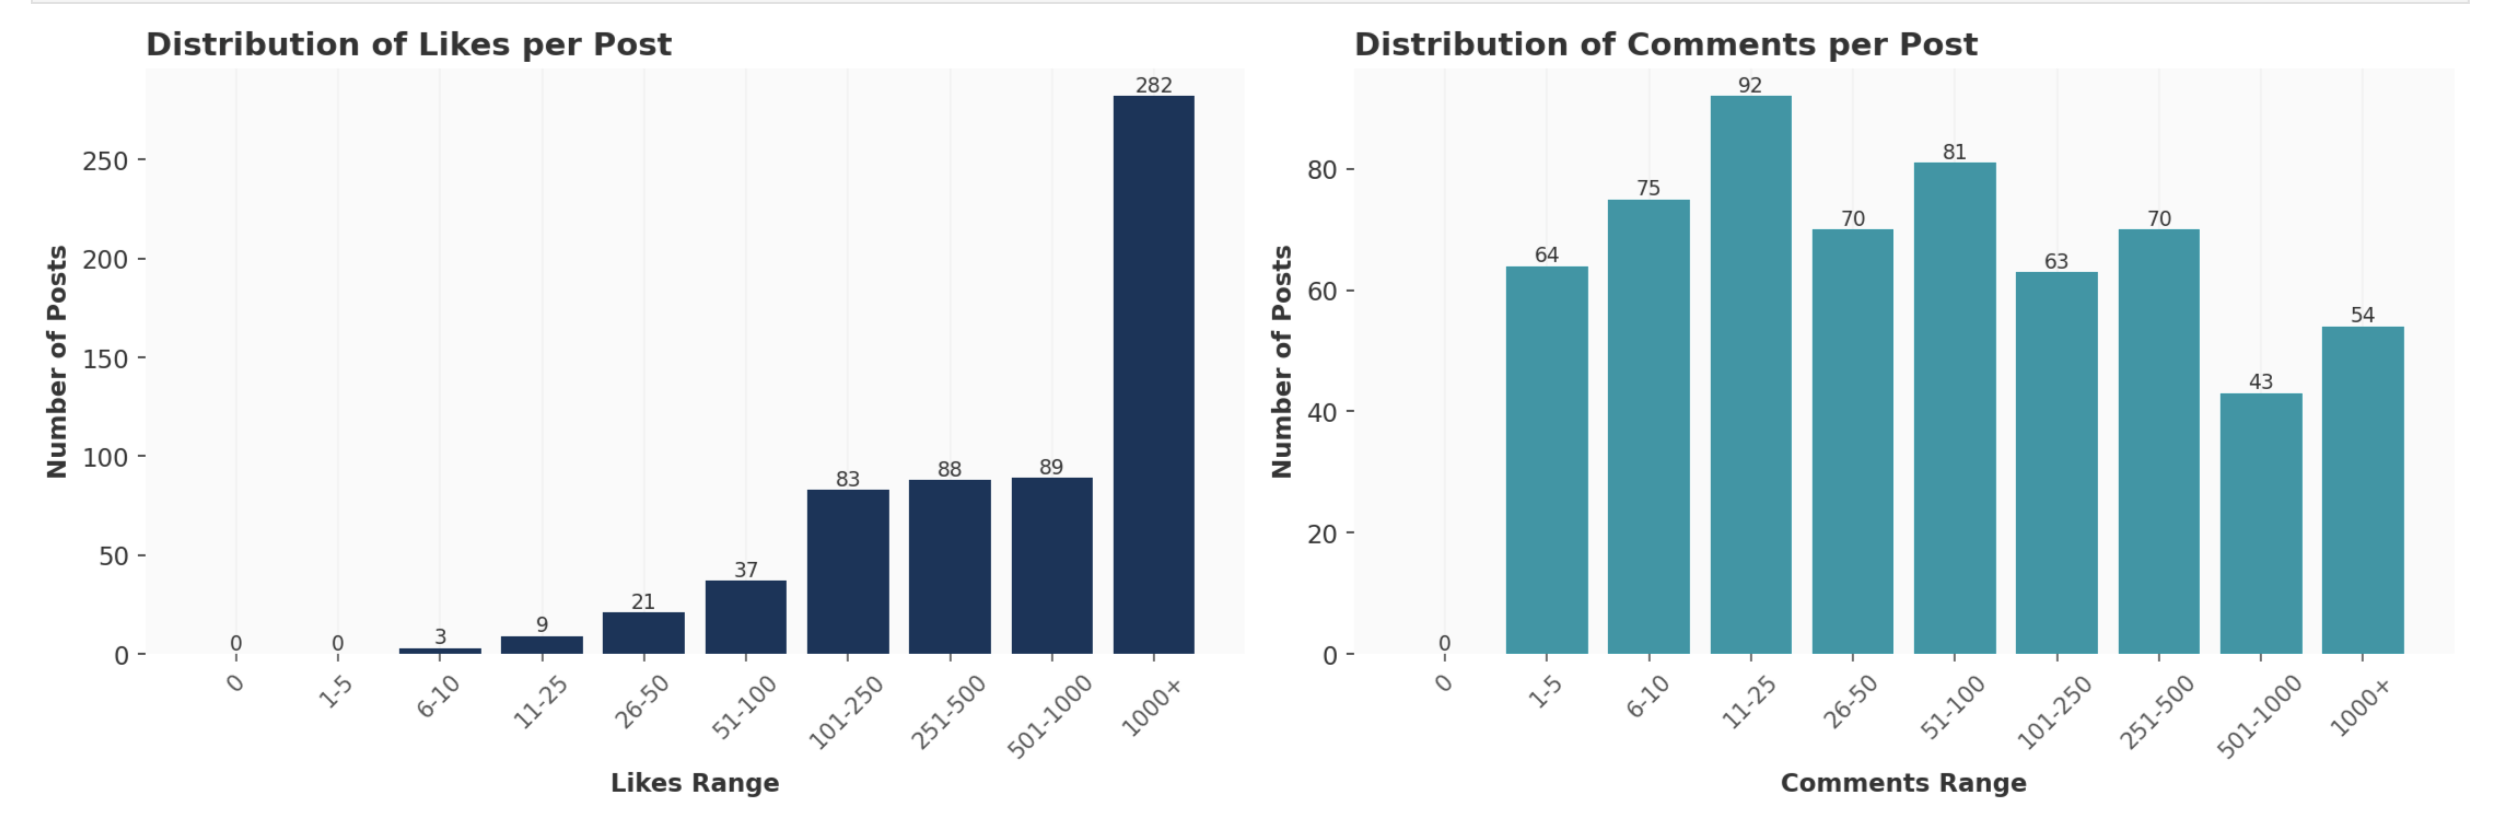
\includegraphics[width=0.9\textwidth]{plots/engagement_distribution.png}
\caption{Distribution of posts according to likes and comments engagement levels.}
\label{fig:engagement_distribution}
\end{figure}

The dataset covers the period from April 2018 to July 2026, encompassing approximately nine years of Instagram activity. This temporal span allows for the examination of variations in posting and interaction patterns over an extended period, while accounting for potential shifts in online discourse and platform dynamics. Figure~\ref{fig:temporal_distribution} presents the temporal distribution of posts included in the dataset.

\begin{figure}[!htbp]
\centering
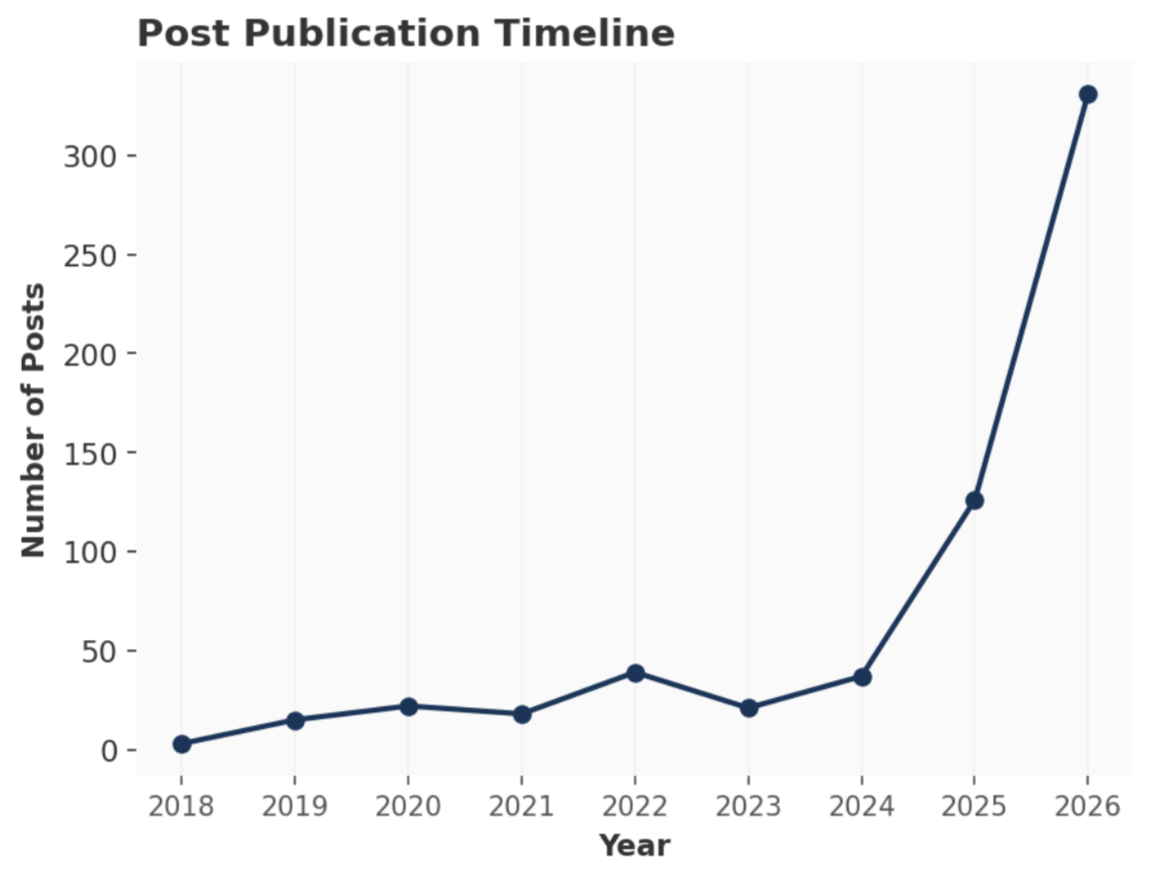
\includegraphics[width=0.85\textwidth]{plots/Post_Publication_timeline.png}
\caption{Temporal distribution of posts in the dataset.}
\label{fig:temporal_distribution}
\end{figure}


Finally, publisher and user verification statuses were analysed to describe the distribution of verified and non-verified accounts within the dataset. At the post level, 414 posts (67.6\%) were published by non-verified accounts, while 198 posts (32.4\%) originated from verified publishers. At the comment level, verified users accounted for only 2.11\% of all interactions, indicating that engagement was predominantly generated by non-verified accounts.


\begin{figure}[!htbp]
\centering
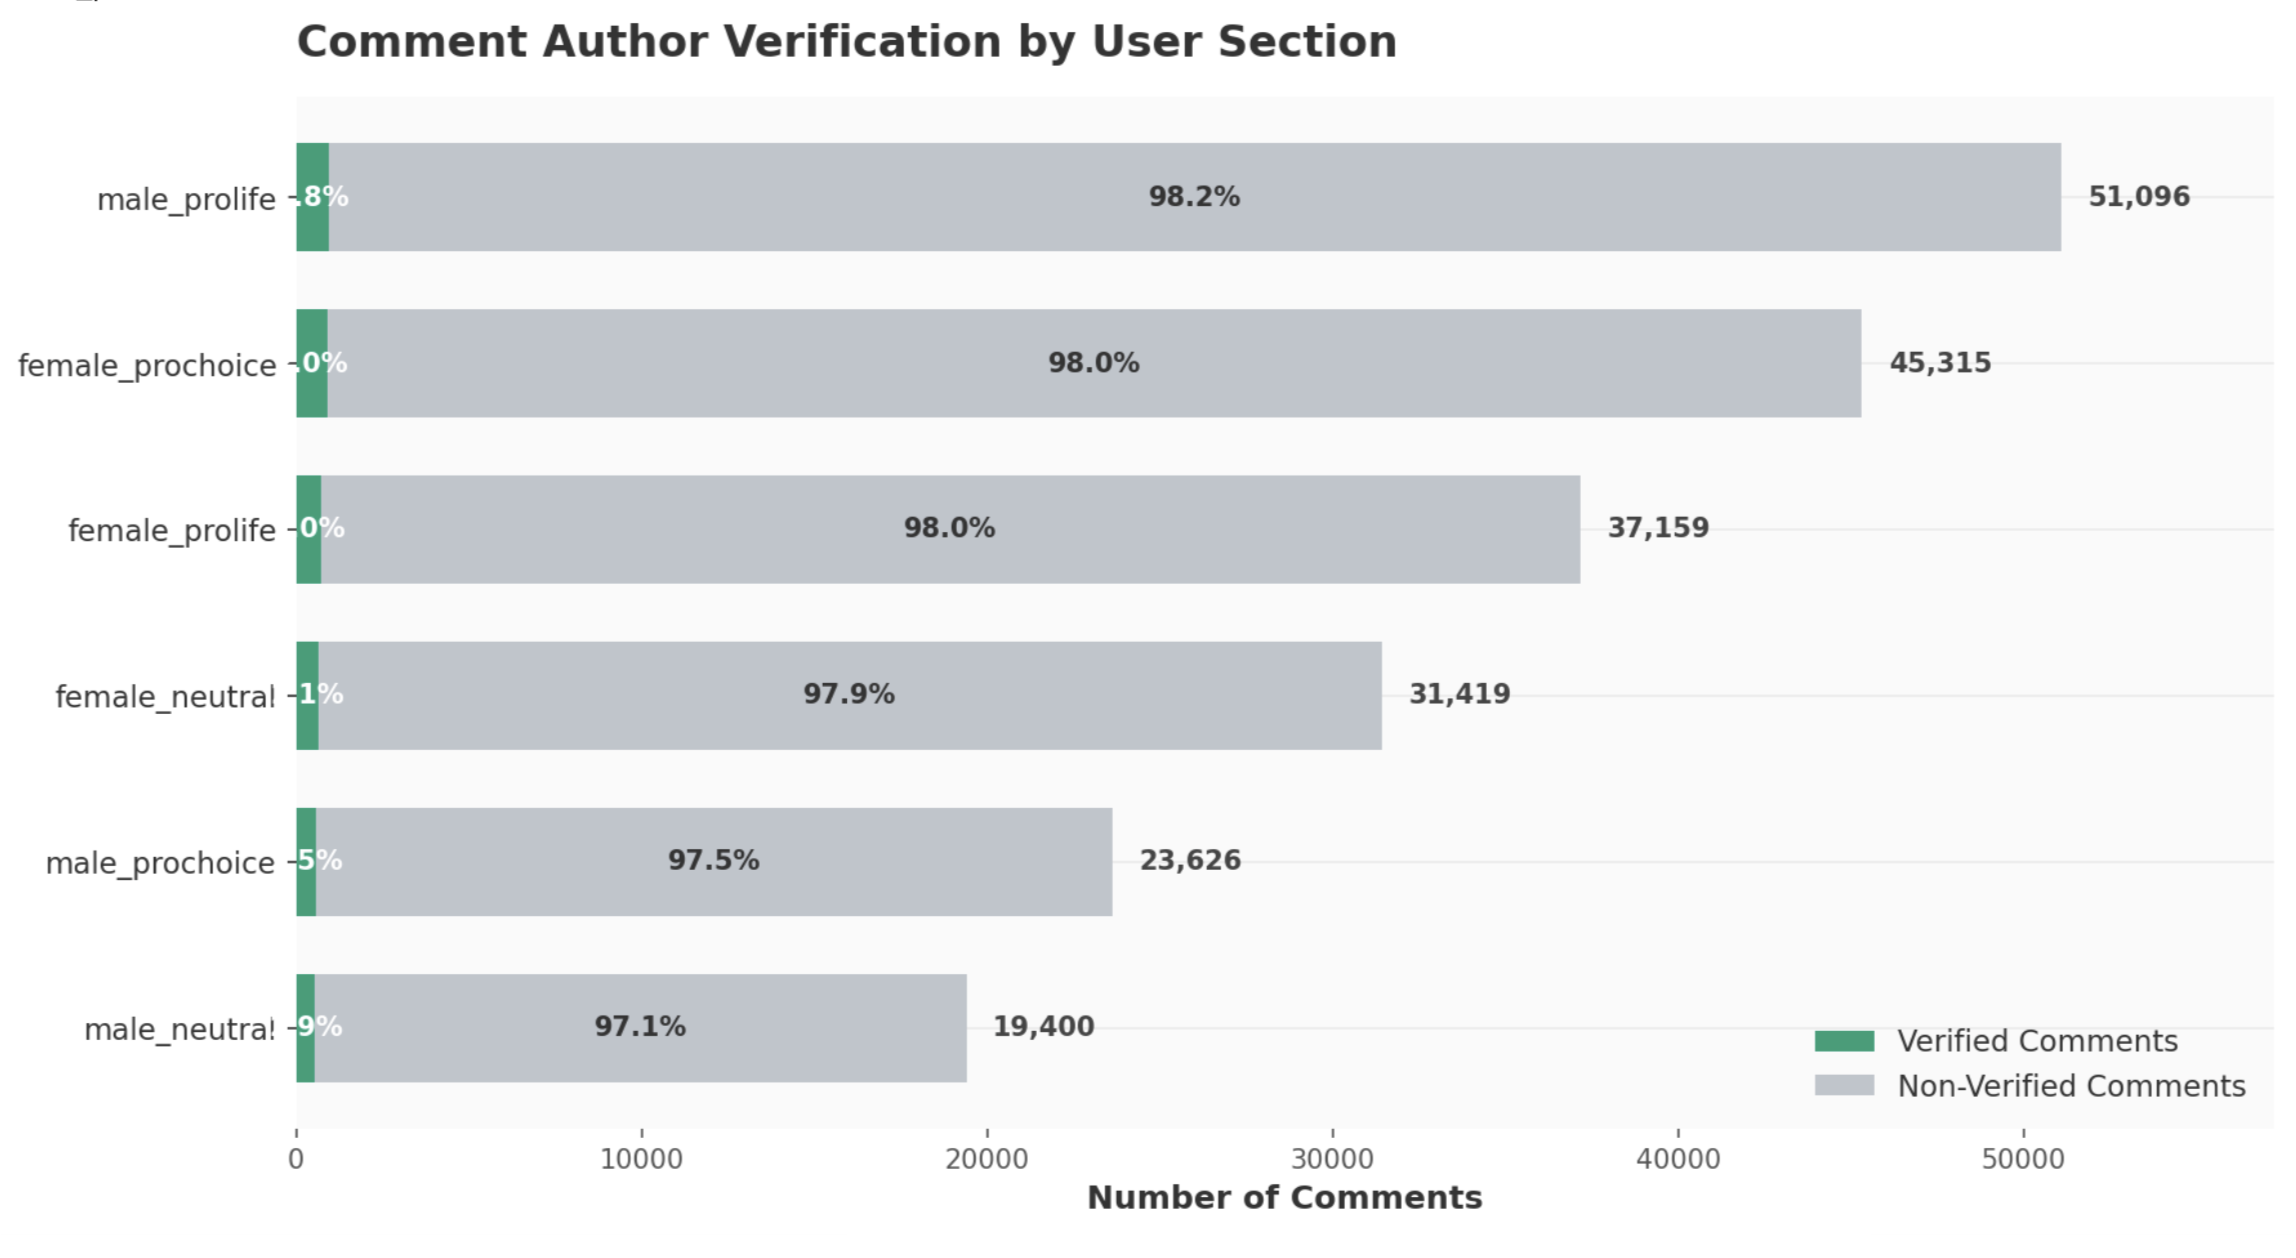
\includegraphics[width=0.9\textwidth]{plots/verification_distribution.png}
\caption{Distribution of verified and non-verified comments across user categories.}
\label{fig:verification_distribution}
\end{figure}

\subsection{Research Objectives}

This study investigates factors influencing divergence in Instagram interactions, specifically examining how engagement metrics, user attributes, and temporal factors relate to divergence scores across different demographic and ideological positions.


\clearpage

\section{Data Collection Methodology}

\subsection{Scraping Process}

Data collection followed a two-stage approach: (1) Selenium-based hashtag exploration to identify relevant Instagram posts across ideological categories, and (2) automated comment extraction using \texttt{instagram\_comment\_scraper.py} with session persistence and resumable operation.

\subsection{Comment Extraction}

The scraper collected post metadata, including URL, timestamp, verification status, total likes, and comment count. At the comment level, it extracted usernames, comment text, like counts, reply counts, and verification status. The system used cookie persistence, SQLite tracking, rate limiting, and scroll-based loading to reliably retrieve dynamically loaded comments.

\subsection{Dataset Composition}

The final dataset contained 3,672 posts, with 612 posts collected from each of the six target categories. This balanced distribution enables comparative analysis across demographic and ideological groups.

\subsection{Rate Limiting and Anti-Detection Measures}

To improve reliability and minimize excessive requests, the scraper used randomized delays, human-like login behaviour, configurable scrolling limits, and cookie-based session reuse.

\subsection{Data Quality Considerations}
Several measures were implemented to ensure the consistency and reliability of the collected dataset. GIF comment verification was performed, as Instagram generates temporary session-specific parameters and expiration timestamps within GIF URLs, causing the same GIF content to appear under different links across requests or page loads. Therefore, GIF comments were identified using additional extracted metadata, including username, like count, and reply information, rather than relying solely on URL comparison. Furthermore, schema-based validation, engagement value standardization, error logging, and reliable storage mechanisms were implemented to maintain data integrity and prevent data loss during interruptions.


\subsection{Ethical Considerations and Data Collection Challenges}

The data collection process followed responsible social media research practices by using only publicly available information, applying rate-limiting measures, minimizing unnecessary requests through session persistence, and avoiding repeated scraping through database tracking.

Several technical challenges were encountered during implementation. Instagram interface changes affected selector reliability, requiring adaptive selectors and fallback methods. Platform restrictions, including rate limits and access blocks, were managed through controlled requests and proxy rotation. Additionally, Instagram's dynamic comment loading introduced variability in extraction results. Since comments are loaded progressively during scrolling, proxy speed, network conditions, and execution time influenced the number of comments collected from each post. This was addressed through resumable scraping and incremental data collection across multiple sessions.

Despite these challenges, the implemented approach enabled the successful collection of a structured dataset for analysing Instagram comment patterns.


\clearpage

\section{User Difference Analysis}









\subsection{Divergence Metrics}

To characterize differences in commenting behaviour between user groups, we examine two complementary dimensions of divergence:\\ \textbf{content divergence}, which captures differences in the composition of comments, and \textbf{order divergence}, which captures differences in the temporal arrangement of comments within discussions.

\medskip

\noindent\textbf{Content divergence:}
\vspace{0.3cm}
\\
Content divergence measures the extent to which two user groups contribute different sets of comments, independent of their ordering. Given two comment multisets $A$ and $B$, we define this measure using their normalized symmetric difference:
\[
D_{\text{cont}}(A,B)=\frac{|A \triangle B|}{|A|+|B|}.
\]



Lower values indicate greater similarity in the types of comments produced by the two groups, whereas higher values indicate more distinct commenting patterns.



\begin{figure}[!htbp]
\centering
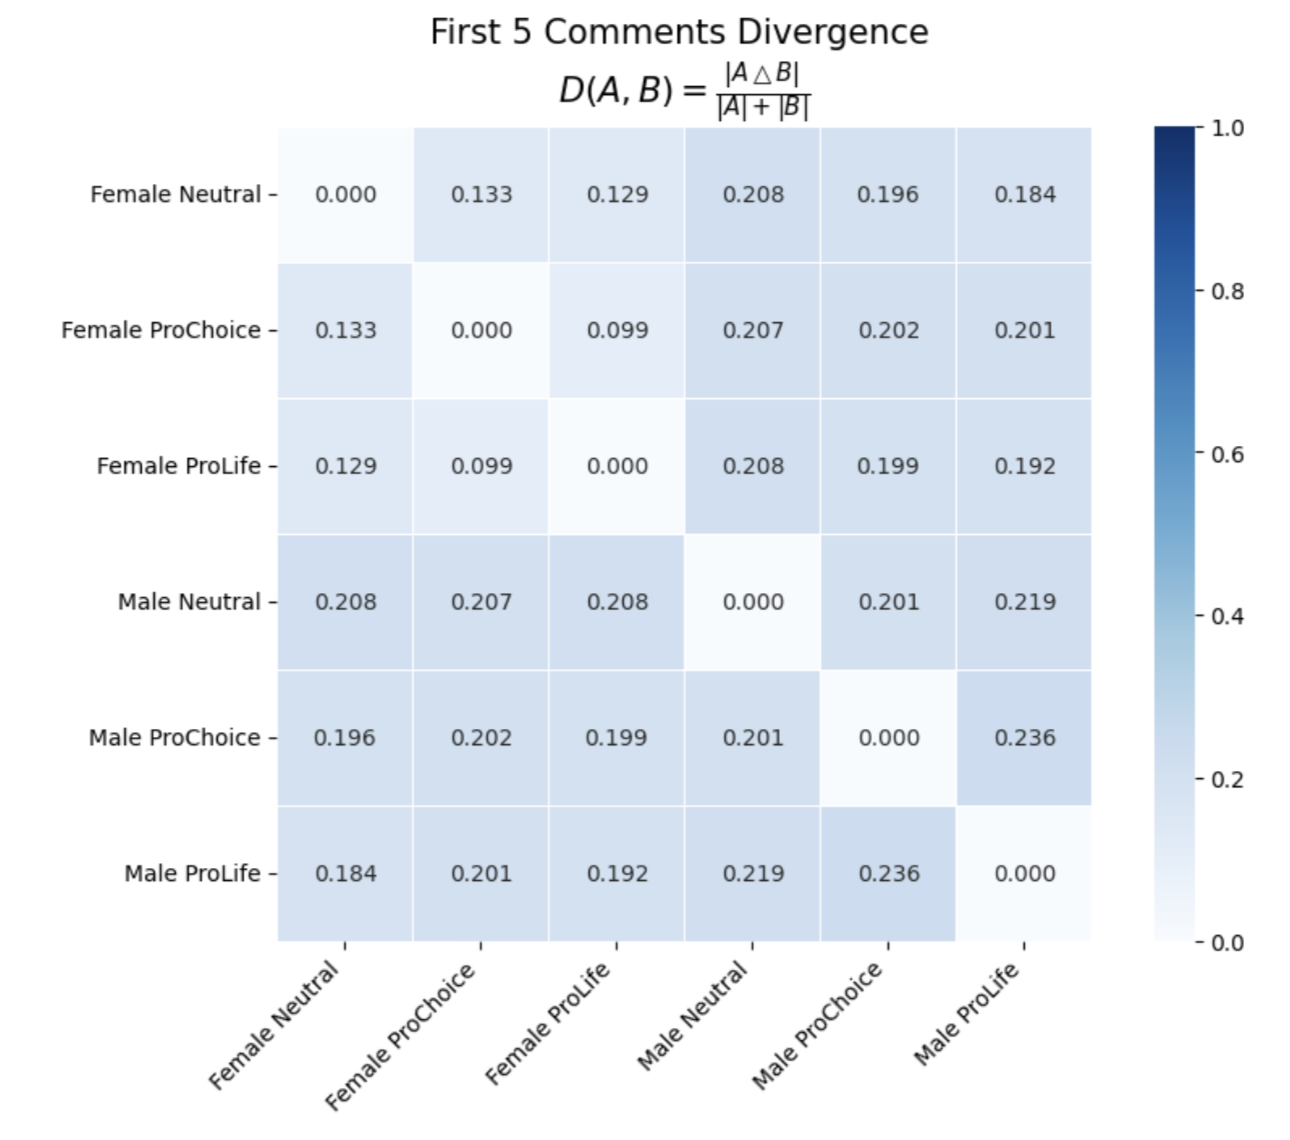
\includegraphics[width=0.65\textwidth]{plots/multiset_divergence_matrix.png}
\caption{Content divergence across user categories based on the first five comments per post.}
\label{fig:multiset_divergence}
\end{figure}

\vspace{1.5cm}

\medskip

\noindent\textbf{Order divergence:}
\vspace{0.5cm}
Beyond differences in comment content, user groups may also differ in how they engage with discussions. Order divergence captures these sequential differences by measuring whether corresponding comments occupy the same positions within discussion threads. For example, which comment appears first, second, and so on.

Formally, given two ordered comment sequences $A$ and $B$ of length $n$, we define:
\[
D_{\text{ord}}(A,B)=\frac{1}{n}\sum_{i=1}^{n}\mathbf{1}_{[A_i \neq B_i]}.
\]
This measure reflects differences in participation dynamics rather than differences in the comments themselves.

\begin{figure}[!htbp]
\centering
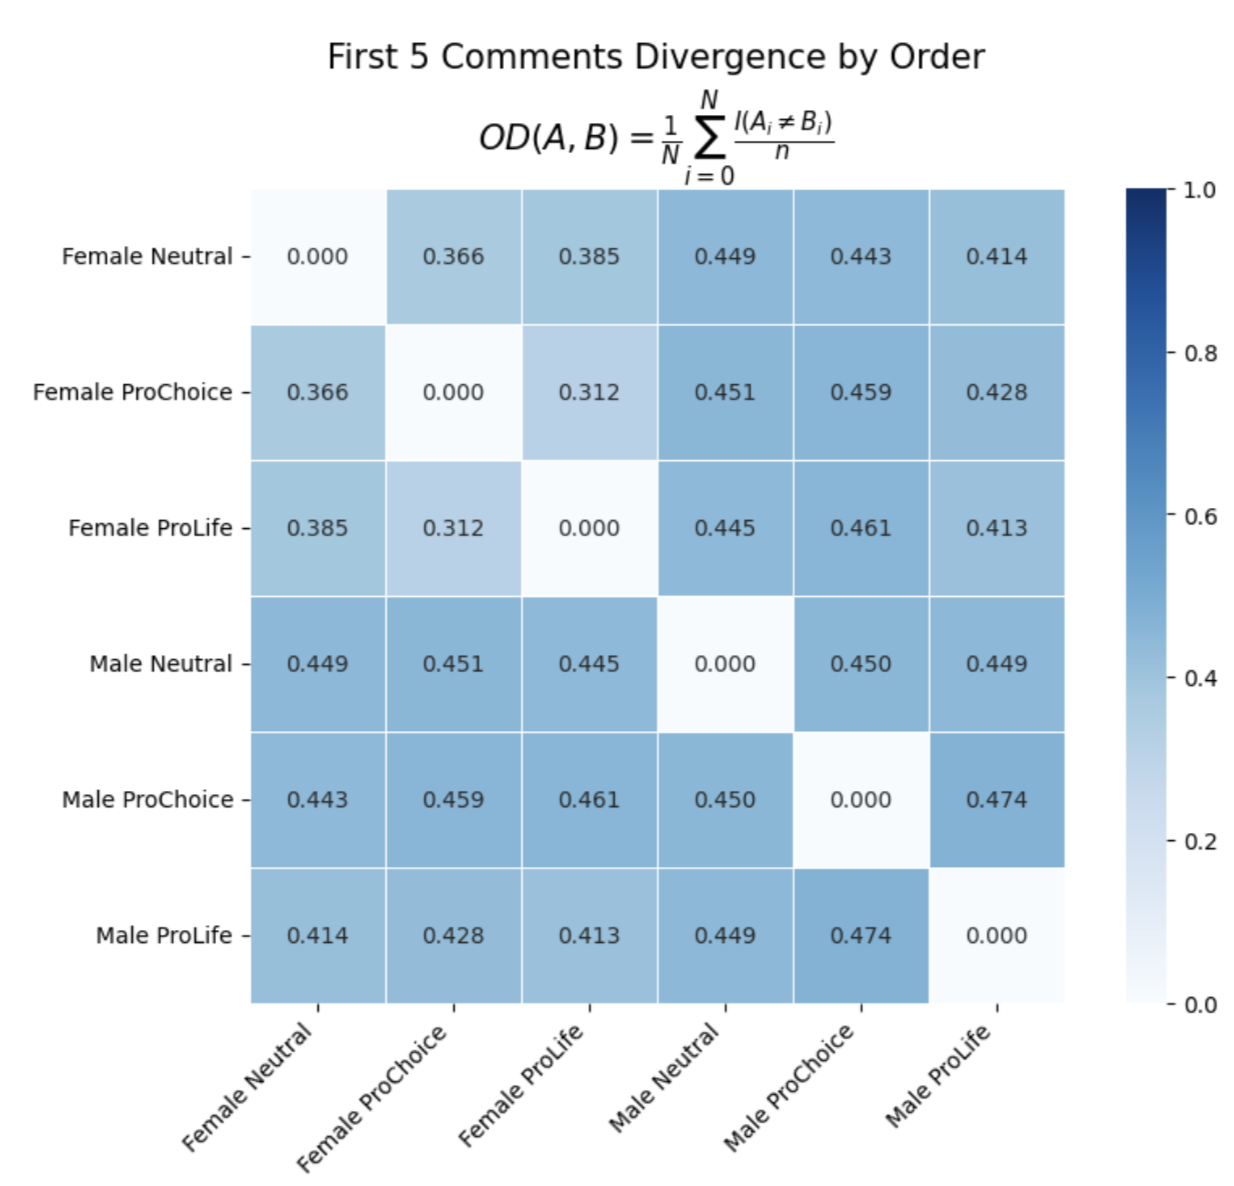
\includegraphics[width=0.65\textwidth]{plots/ordered_divergence_matrix.png}
\caption{Order divergence across user categories based on the first five comments per post.}
\label{fig:ordered_divergence}
\end{figure}
















































\subsection{Comment Depth Effects}

To evaluate how the number of comments considered influences the divergence measures, we progressively increase the comment depth $N$, where $N$ denotes the number of Top comments analysed per post.

\begin{figure}[!htbp]
\centering
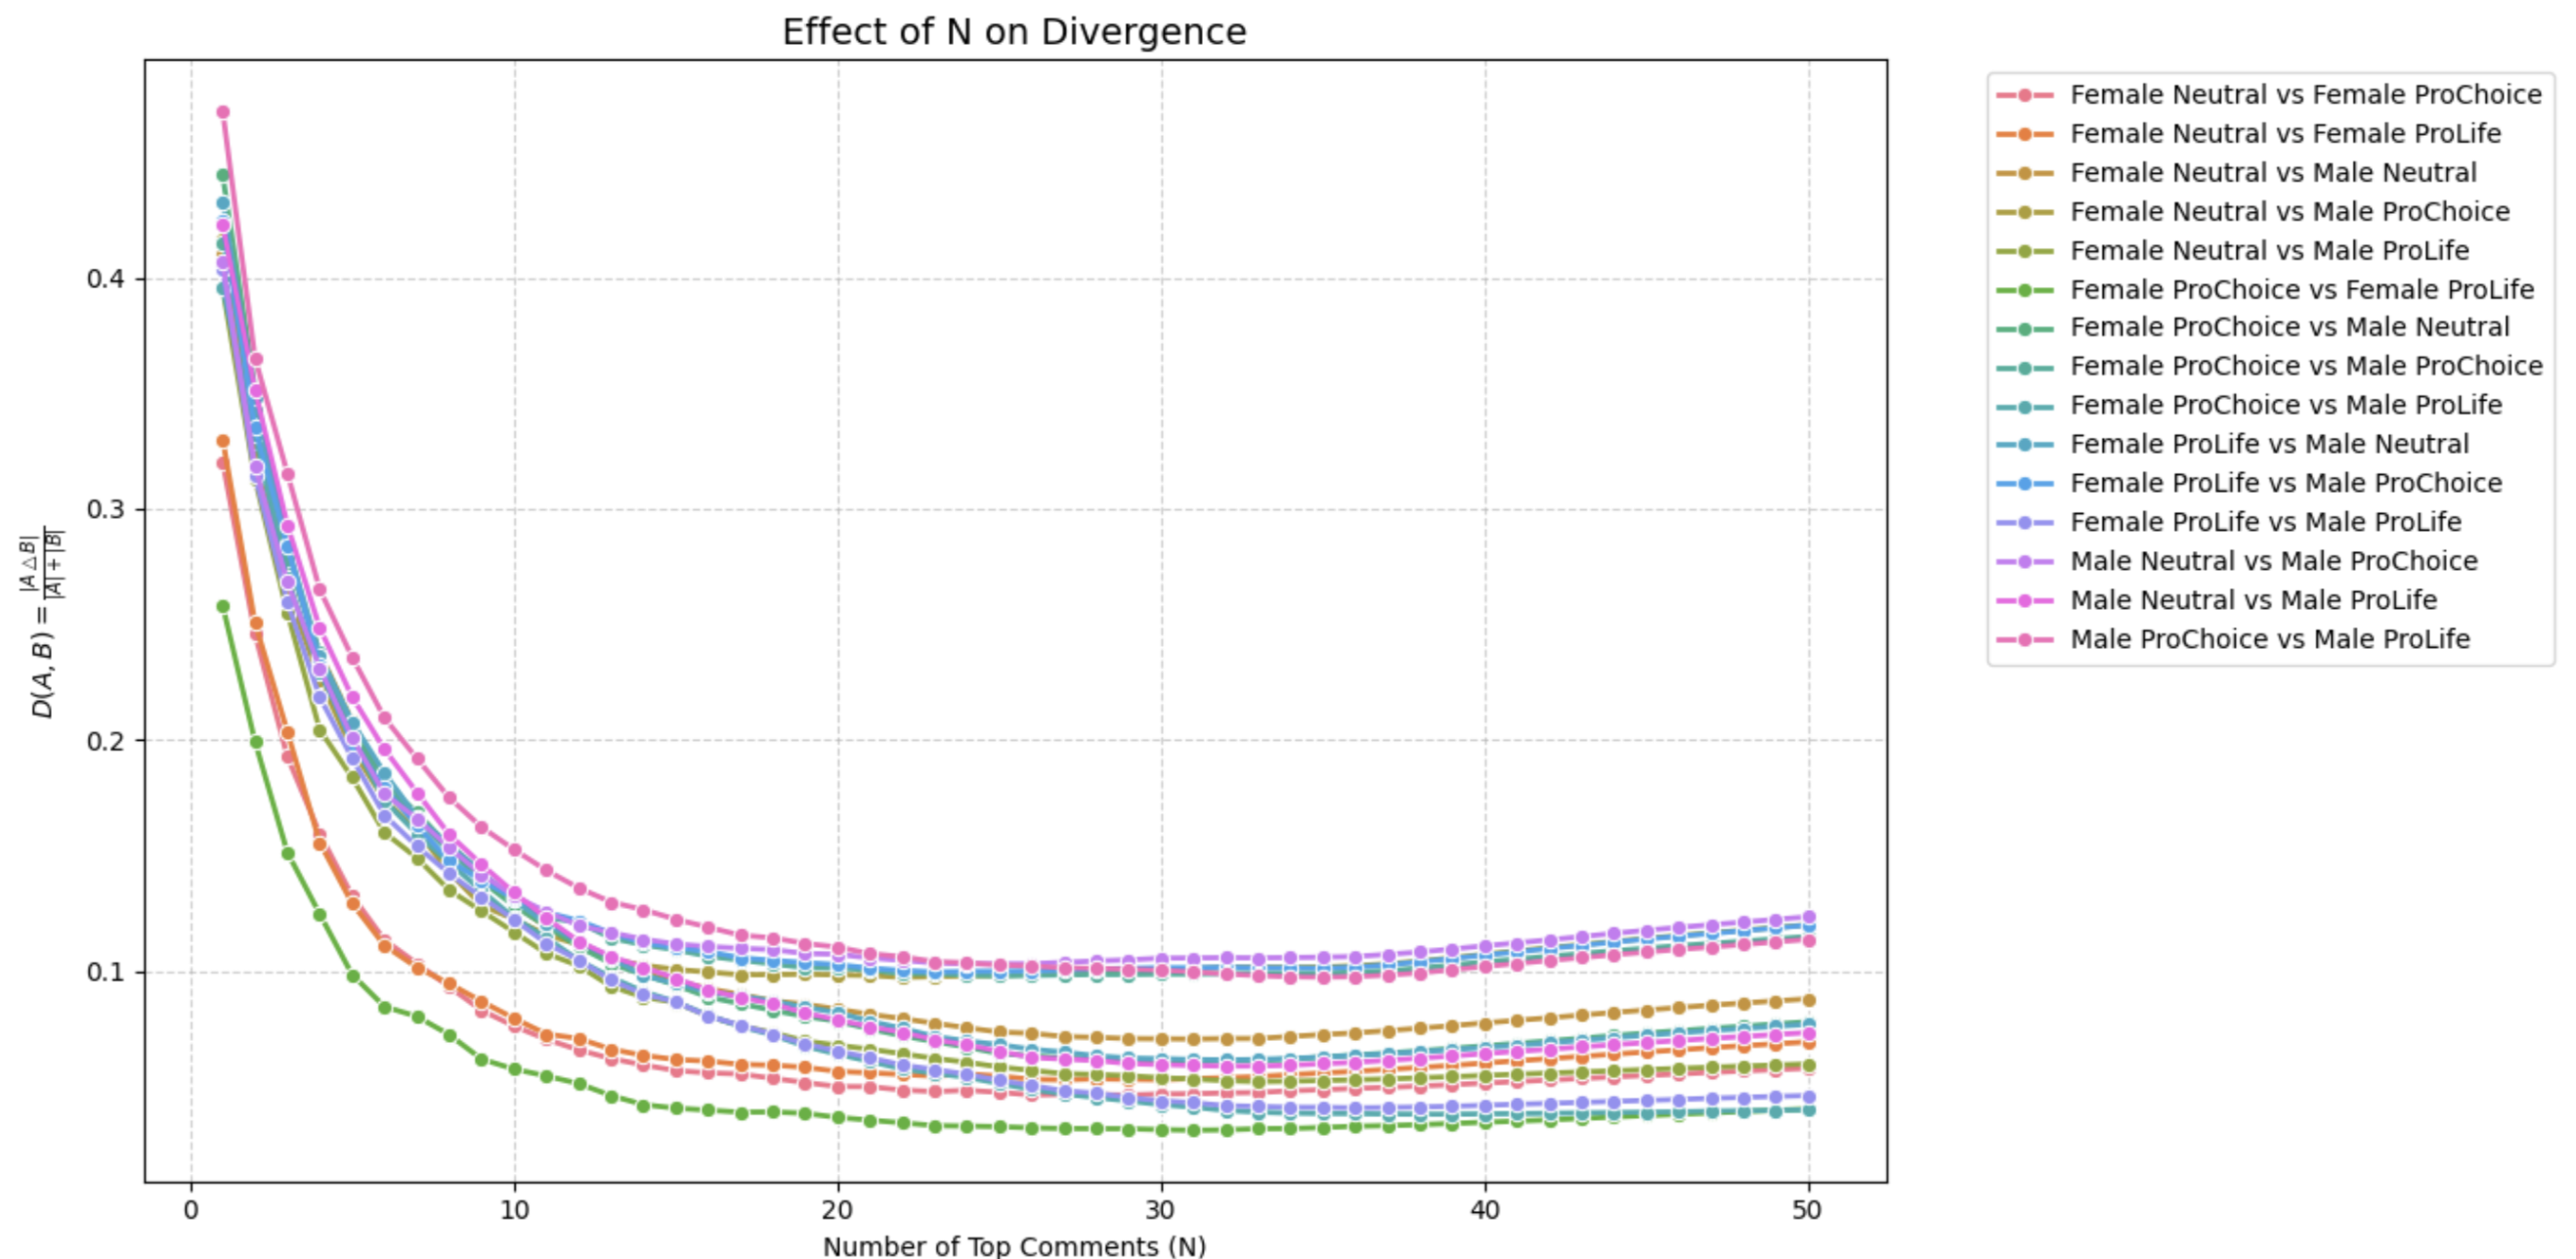
\includegraphics[width=0.75\textwidth]{plots/divergence_vs_n.png}
\caption{Effect of comment depth ($N$) on content divergence.}
\label{fig:divergence_vs_n}
\end{figure}

As shown in Figure~\ref{fig:divergence_vs_n}, content divergence decreases rapidly before converging after approximately 15--20 comments. This suggests that the overall comment composition becomes stable once a sufficient number of comments are included.

\begin{figure}[!htbp]
\centering
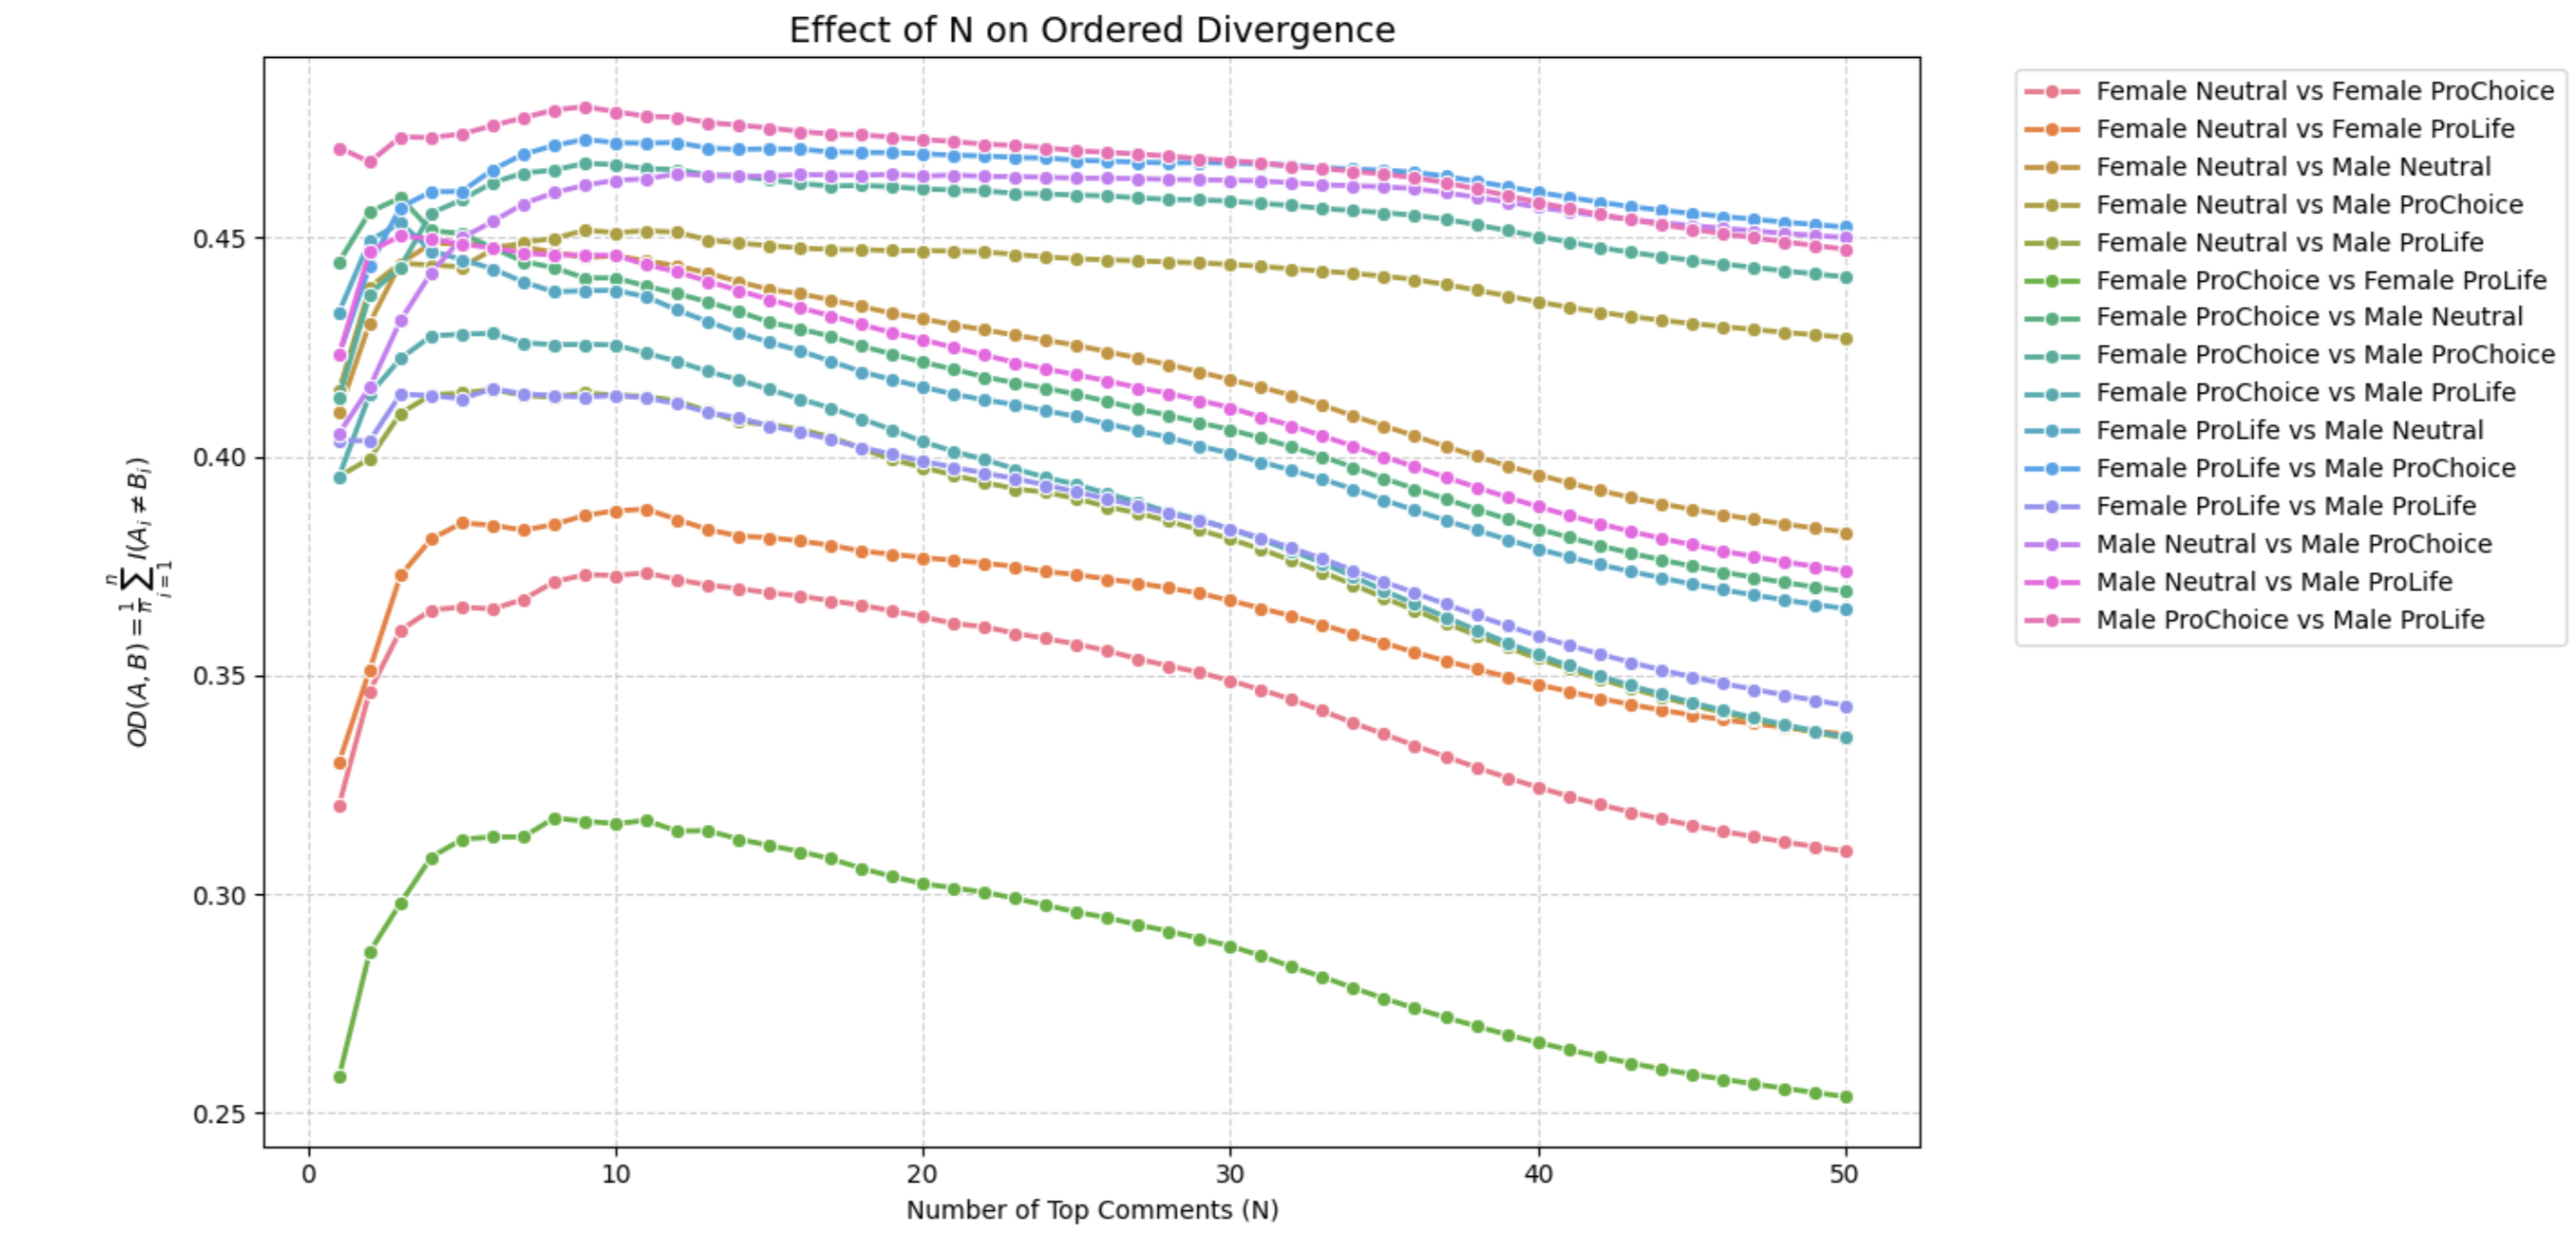
\includegraphics[width=0.75\textwidth]{plots/ordered_divergence_vs_n.png}
\caption{Effect of comment depth ($N$) on ordered divergence.}
\label{fig:ordered_divergence_vs_n}
\end{figure}

In contrast, ordered divergence remains relatively stable across all values of $N$, indicating persistent differences in the temporal ordering of comments. Overall, the results suggest that content differences converge with increasing comment depth, whereas differences in participation dynamics remain consistent throughout the discussion.


\subsection{Discussion}
The divergence analysis shows distinct commenting patterns across user categories. For the first five comments, content divergence is relatively low (0.099--0.236), whereas ordered divergence is considerably higher (0.312--0.474), indicating that differences are more pronounced in participation order than in comment content. The largest divergence is observed between the Male ProChoice and Male ProLife groups, while female groups exhibit the greatest similarity.
These results suggest that commenting behaviour varies across user categories, although the observed differences are likely influenced by additional user- and platform-specific factors beyond gender or stance alone.


\clearpage

\section{Feature Engineering}

\subsection{Dataset Construction}

The dataset was constructed from 612 posts shared across six user categories. All possible category pairs were generated for each post, resulting in:

\[
\binom{6}{2}=15
\]

pairwise interactions per post. Each observation represents a user-category pair and its corresponding divergence score, producing a final dataset of:

\[
612 \times 15 = 9,180
\]

observations.

\subsection{Extracted Features}

The divergence score was used as the target variable. The predictive features were grouped into four categories:

\begin{itemize}
    \item \textbf{Engagement:} \textit{post\_likes}, \textit{post\_comments}, \textit{log\_likes}, \textit{log\_comments}
    \item \textbf{Temporal:} \textit{months\_since\_post}
    \item \textbf{User attributes:} \textit{verified\_encoded}, \textit{gender\_match}
    \item \textbf{Stance interactions:} eight one-hot encoded variables representing user stance-pair combinations
\end{itemize}

\clearpage

\section{Model Comparison: Linear Regression vs. ZOIB}

\subsection{Dataset Characteristics}
The dataset contains 9,180 posts with divergence scores between 0 and 1. The distribution is highly skewed, with 54\% zero divergence, 1.4\% complete divergence, and a mean score of 0.188. The bounded distribution motivates the use of ZOIB regression.

\begin{figure}[!htbp]
\centering
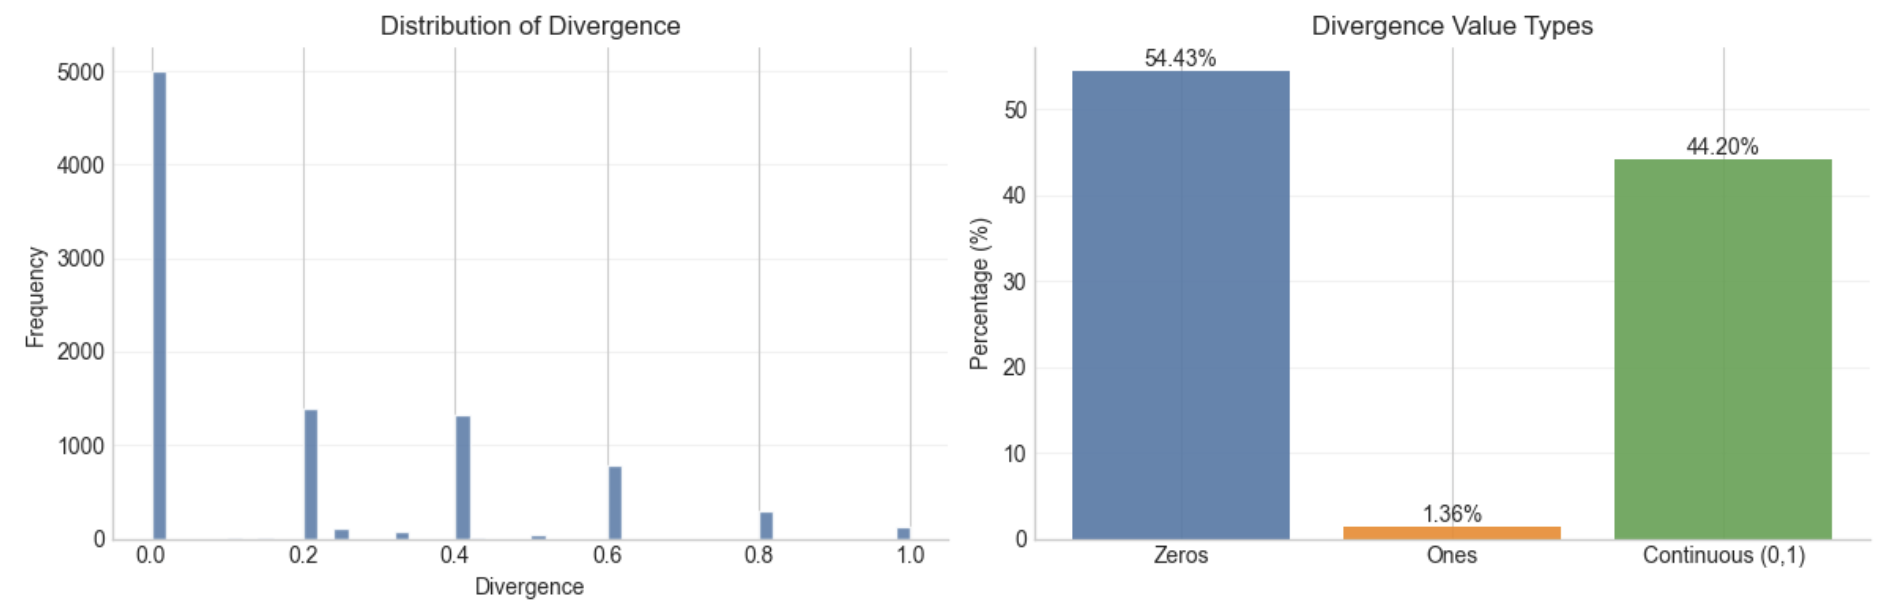
\includegraphics[width=0.8\textwidth]{plots/div_distribution.png}
\caption{Distribution of Divergence }
\label{fig:divergence_distribution}
\end{figure}


\subsection{Linear Regression}

The linear model explained approximately 34\% of the variance in divergence.
The model identified meaningful relationships:
\begin{itemize}
    \item Divergence decreases as post age increases (newer posts exhibit higher divergence).
    \item Posts with a higher total number of comments tend to show more divergence. This is intuitively correct.
\end{itemize}

However, the model shows limited predictive ability. The training and testing set prediction plots are nearly identical, indicating that the model is not overfitting and not underfitting.

\begin{figure}[!htbp]
\centering
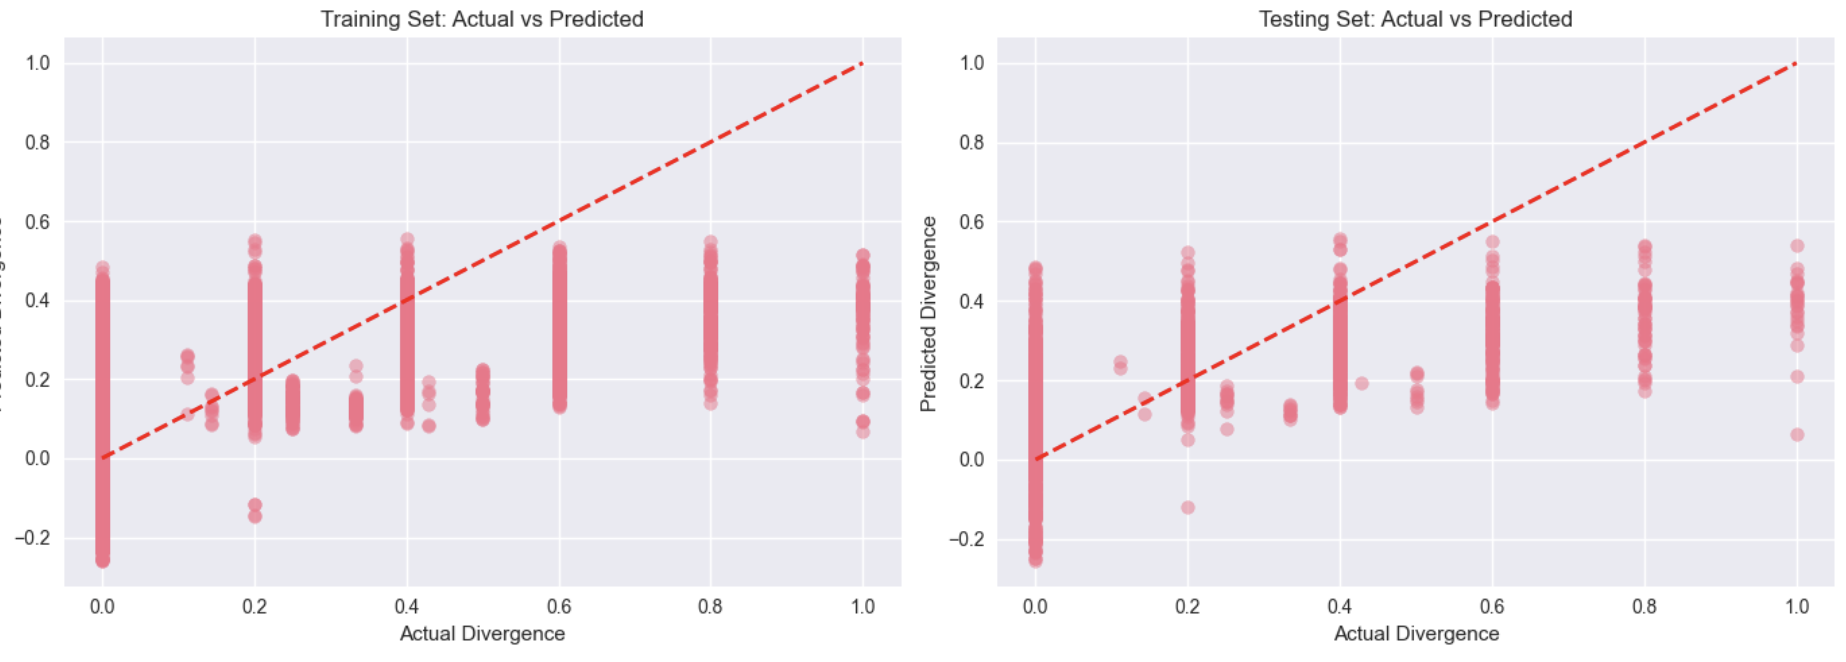
\includegraphics[width=0.8\textwidth]{plots/actual_vs_predicted_linear.png}
\caption{Actual vs. Predicted Divergence for Linear Regression}
\label{fig:linear_actual_predicted}
\end{figure}


Pairwise linear regression across all 15 user-group combinations revealed that the flat, vertically distributed pattern persists uniformly. This demonstrates that the predictive failure is not merely an artifact of grouping multiple classes, but rather stems from an inherent lack of a linear signal in the data, encouraging the use of generalized non-linear modeling and richer feature extraction to capture the underlying variance.



\begin{figure}[!htbp]
\centering
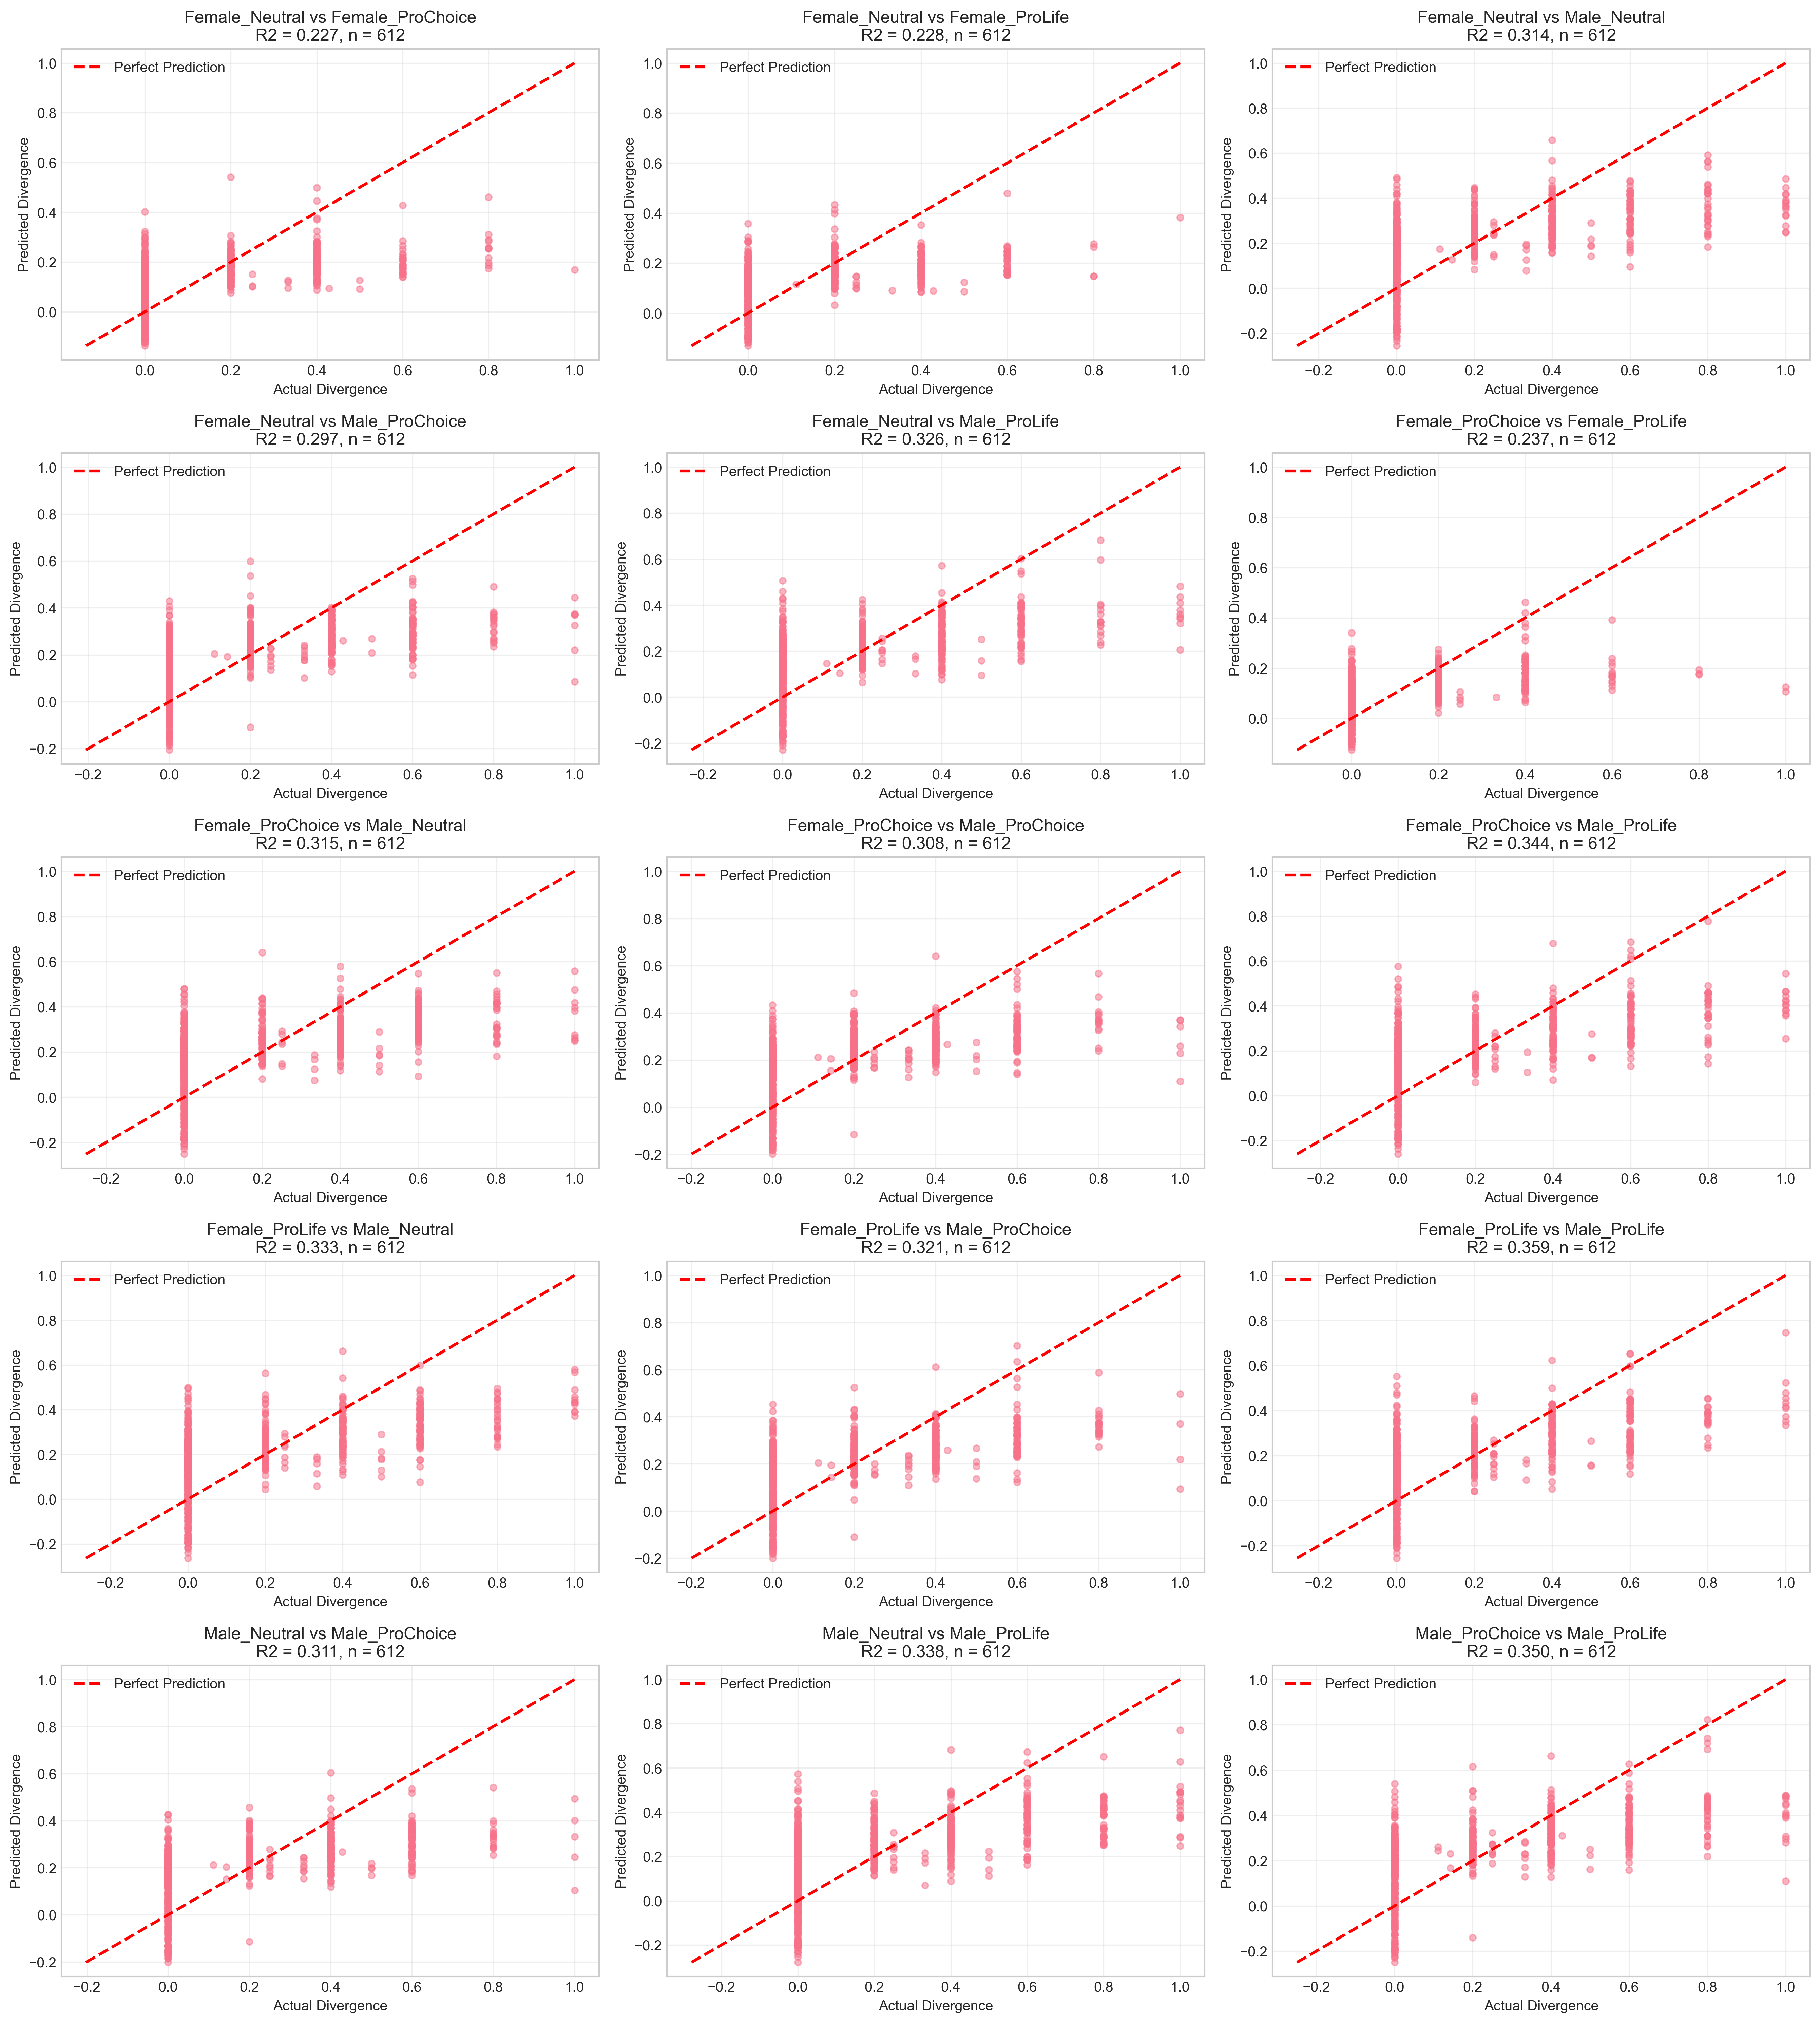
\includegraphics[width=0.8\textwidth]{plots/15_model_predictions.png}
\caption{Actual vs. Predicted Divergence for Pairwise Linear Regression Across the 15 Combinations of 6 User Groups}
\label{fig:linear_15_model_predictions}
\end{figure}

\vspace{1cm}
However, alternative approaches, Ridge, Lasso, and XGBoost, did not meaningfully improve performance. Linear regression performed the same overall, though XGBoost was slightly better but not by much.












\vspace{1cm}


\subsection{Zero-One Inflated Beta (ZOIB) Regression}

The model separates divergence into three distinct processes:
\begin{enumerate}
    \item the probability of zero divergence;
    \item the probability of complete divergence;
    \item the mean divergence for observations strictly between 0 and 1.
\end{enumerate}

The fitted ZOIB model achieved the following predictive performance:

\[
R^2 = 0.4427, \qquad
RMSE = 0.1868, \qquad
MAE = 0.1294.
\]

Compared with the linear regression model, the ZOIB model achieved a higher predictive $R^2$ (0.4427 versus 0.3472), corresponding to an approximate 28\% relative improvement in predictive performance. Because the two models use slightly different predictor sets, this improvement should not be attributed solely to the modelling framework.

\subsection{Performance Comparison}

\begin{table}[H]
\centering
\begin{tabular}{lcc}
\hline
\textbf{Metric} & \textbf{ZOIB} & \textbf{Linear Regression} \\
\hline
$R^2$ & 0.4427 & 0.3472 \\
RMSE & 0.1868 & 0.2022 \\
MAE & 0.1294 & 0.1599 \\
\hline
\end{tabular}
\caption{Predictive performance of the ZOIB and linear regression models.}
\end{table}

\subsection{Feature Interpretation}

Despite their different modelling assumptions, both approaches identified similar overall patterns.

\begin{itemize}
    \item \textbf{Time effect:} Older posts tend to exhibit lower divergence.
    \item \textbf{Engagement effect:} Higher engagement, measured by likes and comments, is associated with greater divergence.
    \item \textbf{Gender effect:} Gender matching is generally associated with lower divergence, although the ZOIB model reveals that its effect differs across the zero-inflation, one-inflation, and continuous components.
\end{itemize}

A key advantage of the ZOIB framework is that it models the mechanisms generating zero divergence, complete divergence, and intermediate divergence separately, providing a more detailed understanding of the response process than ordinary linear regression.

\subsection{Regression Analysis of Presence and Rank Variation}


To formally test which factors are associated with the observed variation, two Bayesian generalized linear mixed models with a beta-binomial likelihood were fit, one for presence variation and one for rank variation. Each observation corresponds to one post and one pairwise account comparison. Fixed effects include the log-standardized number of comments and likes on the post, the log-standardized age of the post at the time of scraping, a non-directional pairwise label for the gender combination of the two accounts being compared (female-female, female-male, or male-male), a non-directional pairwise label for the stance combination of the two accounts (e.g., prolife-prolife, prochoice-prolife, neutral-prochoice), and the political classification assigned to the post itself (pro-life, pro-choice, ambiguous, or abortion-related but not clearly classifiable to either side). A random intercept for post identity was included in both models to account for repeated comparisons drawn from the same post.
Figure 12 shows the posterior estimates for the presence-variation model. Of all the fixed effects considered, only the age of the post shows a 95\% credible interval that clearly excludes zero, with older posts consistently associated with lower presence variation. Neither the account's own gender pairing nor its stance pairing reaches a comparable level of association once post age and engagement metrics are accounted for; the credible intervals for all six stance-pair categories and all three gender-pair categories overlap zero, although the female-female category shows the most negative point estimate among the gender comparisons, consistent with the descriptive pattern seen in Figure 1. Similarly, none of the four levels of the post's own political classification reaches statistical significance in this sample.

\begin{figure}[H]
\centering
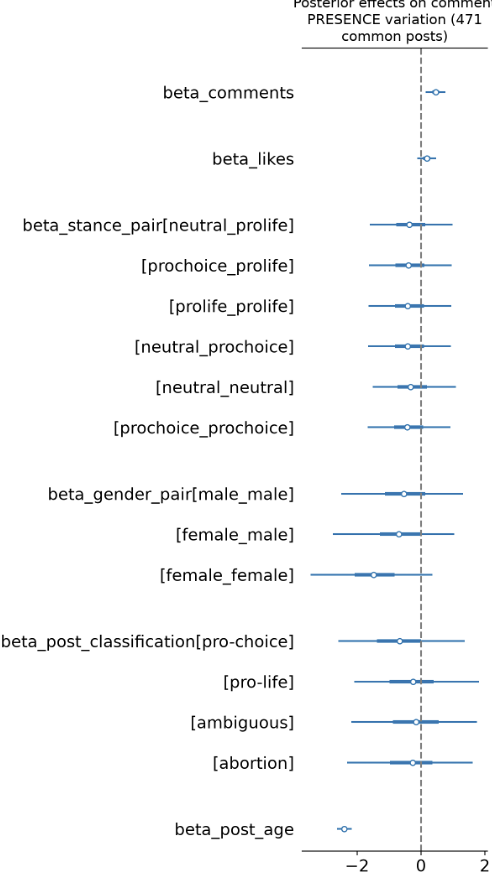
\includegraphics[width=0.8\textwidth]{plots/Posterior_effects_1.png}
\caption{Posterior effects on comment presence variation (471 common posts).}
\end{figure}

Figure 13 shows the corresponding posterior estimates for the rank-variation model. The pattern closely replicates that of the presence-variation model: post age is again the only fixed effect whose 95\% credible interval excludes zero, with the same negative direction, while comment count, like count, gender pairing, stance pairing, and the post's political classification all show credible intervals overlapping zero. As in the presence model, the female-female gender pairing again shows the most negative point estimate of the three gender categories, mirroring the female-pair pattern observed descriptively in Figure 2, though this difference does not reach statistical significance given the width of its credible interval.

\begin{figure}[H]
\centering
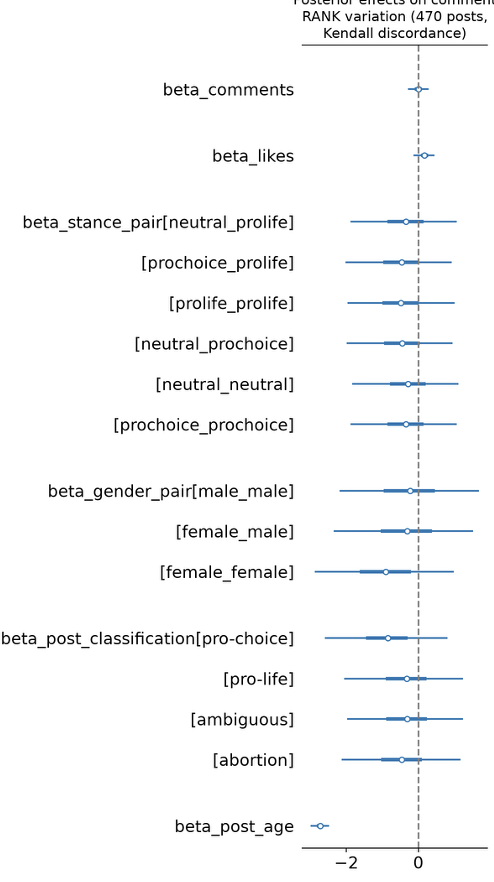
\includegraphics[width=0.8\textwidth]{plots/Posterior_effects_2.png}
\caption{Posterior effects on comment rank variation (470 posts, Kendall discordance).}
\end{figure}

Overall, the regression results indicate that post age is the only variable in either model whose association with comment variation is statistically credible, for both presence and rank-based measures. The political side of the post, the political stance of the viewing accounts, and their gender do not show a statistically credible association with either form of variation once post age and engagement metrics are accounted for, despite the visible gender-related pattern in the descriptive heatmaps.


% References
\clearpage

\section*{References}
\addcontentsline{toc}{section}{References}

\bibliographystyle{apalike}
\bibliography{references}

\end{document}